\section{Diseño de configuraciones}\label{sec:diseno-configuraciones}

\subsection{Política de contraseñas}

Como parte del diseño del servicio de directorio se definió una política de contraseñas centralizada que será aplicada por FreeIPA sobre todas las identidades administradas por la plataforma. El propósito de esta política es establecer requisitos mínimos para la creación, utilización y administración de credenciales, aplicando criterios homogéneos para las cuentas administradas por el servicio de directorio y los servicios integrados.

La definición de la política se fundamenta en los controles establecidos por la norma ISO/IEC 27002:2022, particularmente en los controles 5.17 Información de autenticación (\textit{Authentication Information}) y 8.5 Autenticación segura (\textit{Secure Authentication}) \citep{ISO27002}. El primero establece que la información de autenticación debe controlarse y protegerse a lo largo de su ciclo de vida, abarcando aspectos como su creación, distribución, almacenamiento y renovación, mientras que el segundo exige que las tecnologías y procedimientos de autenticación implementados resistan los intentos de acceso no autorizado y el uso indebido de las credenciales. A partir de estos controles, la política se estructuró en cuatro familias de parámetros: reglas de creación de contraseñas, gestión del ciclo de vida de las credenciales, mecanismos de protección frente a intentos reiterados de acceso y registro de eventos para fines de auditoría.

Considerando las necesidades identificadas durante la fase de análisis, donde se evidenció la ausencia de un estándar institucional para la gestión de contraseñas y la necesidad de adoptar políticas alineadas con estándares internacionales, se definieron los parámetros presentados en la \autoref{tab:password-params}.

\begingroup
\fontsize{8.5pt}{9.5pt}\selectfont
\renewcommand{\arraystretch}{1.3}
\setlength{\tabcolsep}{4pt}

\begin{longtable}{|
>{\raggedright\arraybackslash}p{2.8cm}|
>{\raggedright\arraybackslash}p{3.5cm}|
>{\raggedright\arraybackslash}p{7.2cm}|}

\caption{Parámetros de la política de contraseñas definidos para FreeIPA}
\label{tab:password-params}
\\
\hline
\tableheader
\textbf{Parámetro}                  &
\textbf{Valor definido}             &
\textbf{Justificación}
\\
\hline
\endfirsthead

\caption[]{Parámetros de la política de contraseñas definidos para FreeIPA (continuación)}
\\
\hline
\tableheader
\textbf{Parámetro}                  &
\textbf{Valor definido}             &
\textbf{Justificación}
\\
\hline
\endhead

Longitud mínima                     &
12 caracteres                       &
Incrementa la entropía de las credenciales y dificulta ataques por fuerza bruta.
\\
\hline

Complejidad                         &
Al menos una letra mayúscula, una letra minúscula, un número y un carácter especial &
Reduce la probabilidad de contraseñas predecibles y mejora su resistencia frente a ataques de diccionario.
\\
\hline

Historial de contraseñas            &
5 contraseñas                       &
Evita la reutilización inmediata de credenciales previamente utilizadas.
\\
\hline

Antigüedad mínima                   &
1 día                               &
Impide el cambio reiterado de contraseñas con el propósito de eludir el historial configurado.
\\
\hline

Vigencia máxima                     &
180 días                            &
Favorece la renovación periódica de credenciales sin generar una carga excesiva para los usuarios.
\\
\hline

Intentos fallidos                   &
5                                   &
Reduce el riesgo de ataques automatizados por fuerza bruta.
\\
\hline

Bloqueo de cuenta                   &
5 minutos                           &
Mitiga intentos reiterados de autenticación sin afectar significativamente la disponibilidad del servicio.
\\
\hline

Contraseña temporal                 &
Cambio obligatorio en el primer inicio de sesión &
Garantiza que únicamente el usuario conozca su contraseña definitiva.
\\
\hline

Auditoría                           &
Registro de autenticaciones, cambios de contraseña, bloqueos y restablecimientos &
Permite la trazabilidad de eventos y facilita los procesos de auditoría y respuesta ante incidentes.
\\
\hline
\endlongtable
\endgroup
\normalsize % Restablece explícitamente el tamaño de letra para el texto posterior


Los valores definidos no corresponden a requisitos explícitos establecidos por la norma ISO/IEC 27002:2022, ya que esta específica controles y buenas prácticas, pero no prescribe parámetros concretos como la longitud mínima de las contraseñas o el número máximo de intentos fallidos. En consecuencia, dichos valores fueron determinados como decisiones de diseño considerando las capacidades de configuración ofrecidas por FreeIPA, las recomendaciones internacionales para sistemas de gestión de identidades y el nivel de riesgo identificado para la infraestructura del grupo de investigación \ac{GRID}.

La implementación de esta política permitirá que todos los servicios integrados al directorio compartan un mismo conjunto de reglas de autenticación, eliminando las diferencias existentes entre plataformas y fortaleciendo la gestión centralizada de identidades, la protección de las credenciales y la trazabilidad de los accesos.

\subsection{Diseño del modelo de identidades}

Como parte del diseño del servicio de directorio, es necesario definir la estructura lógica de las identidades que serán administradas por FreeIPA. Esta estructura establece la organización de los usuarios, grupos y cuentas de servicio que posteriormente serán utilizados por las aplicaciones integradas para llevar a cabo los procesos de autenticación y autorización. Esta estructura permite centralizar la gestión de identidades y establecer una fuente común de información para los servicios integrados.

\subsubsection{Definición del nombre de dominio y del \texorpdfstring{\acs{FQDN}}{FQDN}}

Aunque FreeIPA puede integrar un servicio \ac{DNS}, en la presente implementación dicho componente no será utilizado. No obstante, FreeIPA requiere la definición de un nombre de dominio y de un Nombre de Dominio Completamente Calificado (\ac{FQDN}) para el servidor principal, ya que estos identificadores son utilizados por \ac{LDAP}, Kerberos y la infraestructura de certificados digitales para identificar de forma única al servidor y emitir los principales de servicio correspondientes. En atención a este requerimiento, para la infraestructura del grupo \ac{GRID} se definieron el dominio \ac{DNS}, el dominio \ac{LDAP} y el \ac{FQDN} del servidor, tal como se presenta en la \autoref{tab:parametros-implementacion}.

\begingroup
\fontsize{8.5pt}{9.5pt}\selectfont
\renewcommand{\arraystretch}{1.3}
\setlength{\tabcolsep}{4pt}

\begin{longtable}{|
>{\raggedright\arraybackslash}p{2.8cm}|
>{\raggedright\arraybackslash}p{3.8cm}|
>{\raggedright\arraybackslash}p{6.9cm}|}

\caption{Parámetros de dominio y \acs{FQDN} definidos para la infraestructura de FreeIPA}
\label{tab:parametros-implementacion}
\\
\hline
\textbf{Parámetro}                  &
\textbf{Valor definido}             &
\textbf{Justificación}
\\
\hline
\endfirsthead

\hline
\textbf{Parámetro}                  &
\textbf{Valor definido}             &
\textbf{Justificación}
\\
\hline
\endhead

Dominio \acs{DNS}                         &
grid.\allowbreak uniquindio.\allowbreak edu.\allowbreak co &
Corresponde al dominio institucional existente de la infraestructura \ac{GRID}. Este dominio ya es administrado por el servicio \ac{DNS} institucional y únicamente es referenciado por FreeIPA para la construcción de las identidades y de la estructura del directorio.
\\
\hline

Dominio \acs{LDAP} (Base \acs{DN})              &
dc=grid,\allowbreak dc=uniquindio,\allowbreak dc=edu,\allowbreak dc=co &
Se deriva directamente del dominio \ac{DNS}, donde cada componente del nombre de dominio se representa mediante un componente de dominio (Domain Component, dc), conforme al modelo de organización jerárquica utilizado por \ac{LDAP}.
\\
\hline

\acs{FQDN} del servidor                   &
ipa1.\allowbreak grid.\allowbreak uniquindio.\allowbreak edu.\allowbreak co &
Identifica de manera única al servidor FreeIPA dentro de la infraestructura. Este nombre es utilizado por Kerberos para generar los principales de servicio, por la autoridad certificadora para emitir los certificados digitales y por los clientes para establecer conexiones seguras con los servicios proporcionados por FreeIPA.
\\
\hline
\endlongtable
\endgroup
\normalsize % Restablece explícitamente el tamaño de letra para el texto posterior


La selección de estos valores garantiza la coherencia entre los servicios que conforman FreeIPA y evita inconsistencias durante los procesos de autenticación, emisión de certificados y establecimiento de conexiones seguras entre clientes y servidores.

\subsubsection{Definición de la estructura del directorio \texorpdfstring{\acs{LDAP}}{LDAP}}

Una vez definido el dominio de la infraestructura, es necesario establecer la organización lógica de los objetos que serán administrados por FreeIPA. Esta organización corresponde al Árbol de Información del Directorio (\ac{DIT}), el cual define la disposición jerárquica de usuarios, grupos y demás objetos almacenados dentro del servicio \ac{LDAP}. En la solución propuesta se adopta la estructura predeterminada de FreeIPA, la cual organiza los objetos administrativos bajo el contenedor cn=accounts, facilitando la gestión de identidades y proporcionando una estructura consistente para las consultas realizadas por las aplicaciones integradas. La representación de esta estructura se muestra en la \autoref{fig:arbol-directorio}.

\begin{figure}[H]
	\centering
	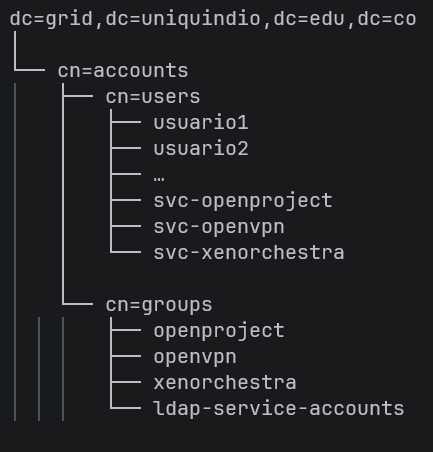
\includegraphics[width=0.6\textwidth]{mainmatter/II-desarrollo-metodologico/disenio/imagenes/arbol-directorio.png}
	\caption{Árbol de información del directorio (\acs{DIT}) definido en FreeIPA}
	\label{fig:arbol-directorio}
\end{figure}

La raíz del árbol corresponde al dominio \ac{LDAP} \nolinkurl{dc=grid,dc=uniquindio,dc=edu,dc=co}, obtenido a partir del dominio institucional. Bajo esta raíz, FreeIPA agrupa los objetos relacionados con la gestión de identidades dentro del contenedor cn=accounts.

El contenedor cn=users almacena tanto las cuentas de los usuarios finales como las cuentas de servicio utilizadas por las aplicaciones para realizar consultas \ac{LDAP}. Por su parte, el contenedor cn=groups reúne los grupos empleados para implementar los mecanismos de autorización de los servicios y para administrar las políticas aplicadas a las cuentas de servicio.

Esta organización constituye la base sobre la cual las aplicaciones realizan las búsquedas \ac{LDAP}. Por ejemplo, los servicios integrados utilizan el contenedor cn=users como punto de partida para localizar usuarios, mientras que la pertenencia a los grupos definidos en cn=groups permite determinar los permisos de acceso correspondientes a cada aplicación.

\subsubsection{Definición de grupos de autorización}

Con el propósito de centralizar la administración del acceso a las aplicaciones integradas, se definieron grupos específicos dentro del directorio para cada uno de los servicios que consumen información desde FreeIPA. En lugar de asignar permisos individualmente a cada usuario, el acceso a las aplicaciones se determina mediante la pertenencia a dichos grupos, tal como se presenta en la \autoref{tab:grupos-autorizacion}.

\begingroup
\fontsize{8.5pt}{9.5pt}\selectfont
\renewcommand{\arraystretch}{1.3}
\setlength{\tabcolsep}{4pt}

\begin{longtable}{|
>{\raggedright\arraybackslash}p{2.8cm}|
>{\raggedright\arraybackslash}p{3.5cm}|
>{\raggedright\arraybackslash}p{7.2cm}|}

\caption{Grupos de autorización.}
\label{tab:grupos-autorizacion}
\\
\hline
\tableheader
\textbf{Grupo}                  &
\textbf{Servicio asociado}     &
\textbf{Propósito}
\\
\hline
\endfirsthead

\hline
\tableheader
\textbf{Grupo}                  &
\textbf{Servicio asociado}     &
\textbf{Propósito}
\\
\hline
\endhead

openproject                         &
OpenProject                         &
Autoriza el acceso a la plataforma de gestión de proyectos mediante autenticación \ac{LDAP}.
\\
\hline

openvpn                             &
OpenVPN                             &
Autoriza a los usuarios que pueden establecer conexiones \ac{VPN} con la infraestructura.
\\
\hline

xenorchestra                        &
Xen Orchestra                       &
Autoriza el acceso a la plataforma de administración de virtualización.
\\
\hline
\endlongtable
\endgroup
\normalsize


Cada servicio realiza consultas \ac{LDAP} filtrando los usuarios pertenecientes al grupo correspondiente, implementando un mecanismo de autorización basado en grupos. Esta estrategia simplifica la administración de permisos, ya que el alta o baja de un usuario únicamente requiere modificar su pertenencia al grupo respectivo sin necesidad de reconfigurar cada aplicación.

\subsubsection{Diseño de cuentas de servicio}

Las aplicaciones integradas requieren realizar consultas al directorio \ac{LDAP} para localizar la información del usuario y establecer el proceso de autenticación. Con este propósito se definieron cuentas de servicio, las cuales son utilizadas exclusivamente por las aplicaciones para establecer la conexión con el directorio y realizar operaciones de consulta. Estas cuentas poseen únicamente los privilegios necesarios para leer la información almacenada en el servicio de directorio, en concordancia con el principio de mínimo privilegio.

Con el fin de mejorar el aislamiento de credenciales y la trazabilidad de las operaciones realizadas sobre el directorio, se definió una cuenta de servicio independiente para cada una de las aplicaciones integradas. Esta estrategia permite administrar las credenciales de forma individual, de manera que un eventual compromiso o rotación de la contraseña de una cuenta no afecte el funcionamiento de los demás servicios. Las cuentas de servicio definidas se presentan en la \autoref{tab:cuentas-servicio}.

\begingroup
\fontsize{8.5pt}{9.5pt}\selectfont
\renewcommand{\arraystretch}{1.3}
\setlength{\tabcolsep}{4pt}

\begin{longtable}{|
>{\raggedright\arraybackslash}p{6.0cm}|
>{\raggedright\arraybackslash}p{7.5cm}|}

\caption{Cuentas de servicio.}
\label{tab:cuentas-servicio}
\\
\hline
\rowcolor[gray]{0.85}
\textbf{Cuenta}                  &
\textbf{Servicio}
\\
\hline
\endfirsthead

\hline
\rowcolor[gray]{0.85}
\textbf{Cuenta}                  &
\textbf{Servicio}
\\
\hline
\endhead

svc-openproject                     &
OpenProject                         \\
\hline

svc-openvpn                         &
OpenVPN                             \\
\hline

svc-xenorchestra                    &
Xen Orchestra                       \\
\hline
\endlongtable
\endgroup
\normalsize


Con el propósito de simplificar la administración de las cuentas de servicio, todas ellas se agrupan en el grupo ldap-service-accounts. Sobre este grupo se aplica una política de contraseñas específica para cuentas de servicio, de modo que toda cuenta incorporada al grupo queda sujeta automáticamente a dicha política, sin necesidad de configurarla de forma individual.

Con el fin de establecer que esta política prevalezca sobre la política global del dominio, se le asigna una prioridad numérica superior. De esta manera, cuando una cuenta pertenece al grupo ldap-service-accounts, FreeIPA aplica la política específica para cuentas de servicio en lugar de la política general utilizada para los usuarios finales.

La política de contraseñas definida para el grupo ldap-service-accounts se resume en la \autoref{tab:politica-service-accounts}

\begingroup
\fontsize{8.5pt}{9.5pt}\selectfont
\renewcommand{\arraystretch}{1.3}
\setlength{\tabcolsep}{4pt}

\begin{longtable}{|
>{\raggedright\arraybackslash}p{3.5cm}|
>{\raggedright\arraybackslash}p{10.0cm}|}

\caption{Política de contraseñas para el grupo ldap-service-accounts.}
\label{tab:politica-service-accounts}
\\
\hline
\rowcolor[gray]{0.85}
\textbf{Elemento}               &
\textbf{Descripción}
\\
\hline
\endfirsthead

\hline
\rowcolor[gray]{0.85}
\textbf{Elemento}               &
\textbf{Descripción}
\\
\hline
\endhead

Grupo                           &
ldap-service-accounts           \\
\hline

Propósito                       &
Agrupar las cuentas de servicio utilizadas por las aplicaciones integradas. \\
\hline

Miembros                        &
svc-openproject, svc-openvpn y svc-xenorchestra. \\
\hline

Política asociada              &
Política de contraseña para cuentas de servicio. \\
\hline

Prioridad                       &
10                              \\
\hline

Configuración principal        &
Contraseña sin expiración.      \\
\hline

Justificación                   &
Evitar la expiración de las credenciales utilizadas por las integraciones, reduciendo la necesidad de intervención administrativa asociada a la renovación de estas cuentas y manteniendo separadas sus políticas respecto de las aplicadas a los usuarios finales. \\
\hline
\endlongtable
\endgroup
\normalsize


La utilización de un grupo dedicado para las cuentas de servicio permite centralizar la administración de las políticas de seguridad y facilita la incorporación de nuevas aplicaciones al servicio de directorio, ya que únicamente es necesario crear la cuenta correspondiente y asociarla al grupo definido.

En conjunto, la estructura del directorio, los grupos de autorización y las cuentas de servicio definen el modelo de gestión de identidades de la solución propuesta. Esta organización centraliza la administración de usuarios y credenciales, facilita la incorporación de nuevos servicios al directorio y define los elementos necesarios para implementar las integraciones \ac{LDAP} descritas en el capítulo de implementación.

\subsection{Definición de máquinas virtuales}\label{subsec:definicion-maquinas-virtuales}

Con el fin de proporcionar redundancia y favorecer la disponibilidad y continuidad del servicio de directorio, la arquitectura propuesta contempla el despliegue de dos servidores FreeIPA: un servidor principal y un servidor réplica. Esta configuración permite mantener una copia sincronizada de la información de identidades, políticas y servicios de autenticación, orientada a proporcionar tolerancia a fallos y continuidad operativa ante la indisponibilidad de uno de los servidores.

Ambas máquinas virtuales fueron diseñadas con características de hardware homogéneas para asegurar un comportamiento consistente durante los procesos de replicación y administración del servicio. Asimismo, los dos servidores ejecutan la misma distribución del sistema operativo y la misma versión de FreeIPA, reduciendo posibles problemas de compatibilidad durante la sincronización de datos. Las especificaciones técnicas de cada servidor FreeIPA se presentan en la \autoref{tab:ficha-servidor-principal} y la \autoref{tab:ficha-servidor-replica}.

\begingroup
\fontsize{8.5pt}{9.5pt}\selectfont
\renewcommand{\arraystretch}{1.3}
\setlength{\tabcolsep}{4pt}

\begin{longtable}{|
	>{\raggedright\arraybackslash}p{4.0cm}|
	>{\raggedright\arraybackslash}p{9.5cm}|}

	\caption{Ficha técnica del servidor principal FreeIPA}
	\label{tab:ficha-servidor-principal}
	\\
	\hline
	\rowcolor[gray]{0.85}
	\textbf{Característica}        &
	\textbf{Especificación}
	\\
	\hline
	\endfirsthead

	\hline
	\rowcolor[gray]{0.85}
	\textbf{Característica}        &
	\textbf{Especificación}
	\\
	\hline
	\endhead

	Nombre de la máquina           & ipa1                                                                        \\ \hline
	Función                        & Servidor principal FreeIPA                                                  \\ \hline
	Sistema operativo              & Fedora Server 44                                                            \\ \hline
	Plataforma de virtualización   & XCP-ng                                                                      \\ \hline
	vCPU                           & 2                                                                           \\ \hline
	Memoria \acs{RAM}              & 4 \acs{GB}                                                                  \\ \hline
	Almacenamiento                 & 50 \acs{GB}                                                                 \\ \hline
	Dirección \acs{IP}             & 172.30.30.61                                                                \\ \hline
	Nombre virtual                 & ipa.\allowbreak grid.\allowbreak uniquindio.\allowbreak edu.\allowbreak co  \\ \hline
	Nombre de dominio (\acs{FQDN}) & ipa1.\allowbreak grid.\allowbreak uniquindio.\allowbreak edu.\allowbreak co \\ \hline
	Dominio IPA                    & grid.\allowbreak uniquindio.\allowbreak edu.\allowbreak co                  \\ \hline
	Reino Kerberos                 & \acs{GRID}.\allowbreak UNIQUINDIO.\allowbreak EDU.\allowbreak CO            \\ \hline
\end{longtable}
\endgroup
\normalsize

\begingroup
\fontsize{8.5pt}{9.5pt}\selectfont
\renewcommand{\arraystretch}{1.3}
\setlength{\tabcolsep}{4pt}

\begin{longtable}{|
	>{\raggedright\arraybackslash}p{4.0cm}|
	>{\raggedright\arraybackslash}p{9.5cm}|}

	\caption{Ficha técnica del servidor réplica FreeIPA}
	\label{tab:ficha-servidor-replica}
	\\
	\hline
	\rowcolor[gray]{0.85}
	\textbf{Característica}        &
	\textbf{Especificación}
	\\
	\hline
	\endfirsthead

	\hline
	\rowcolor[gray]{0.85}
	\textbf{Característica}        &
	\textbf{Especificación}
	\\
	\hline
	\endhead

	Nombre de la máquina           & ipa2                                                                        \\ \hline
	Función                        & Servidor réplica FreeIPA                                                    \\ \hline
	Sistema operativo              & Fedora Server 44                                                            \\ \hline
	Plataforma de virtualización   & XCP-ng                                                                      \\ \hline
	vCPU                           & 2                                                                           \\ \hline
	Memoria \acs{RAM}              & 4 \acs{GB}                                                                  \\ \hline
	Almacenamiento                 & 50 \acs{GB}                                                                 \\ \hline
	Dirección \acs{IP}             & 172.30.30.62                                                                \\ \hline
	Nombre virtual                 & ipa.\allowbreak grid.\allowbreak uniquindio.\allowbreak edu.\allowbreak co  \\ \hline
	Nombre de dominio (\acs{FQDN}) & ipa2.\allowbreak grid.\allowbreak uniquindio.\allowbreak edu.\allowbreak co \\ \hline
	Dominio IPA                    & grid.\allowbreak uniquindio.\allowbreak edu.\allowbreak co                  \\ \hline
	Reino Kerberos                 & \acs{GRID}.\allowbreak UNIQUINDIO.\allowbreak EDU.\allowbreak CO            \\ \hline
\end{longtable}
\endgroup
\normalsize


Las características de hardware de los servidores FreeIPA fueron seleccionadas considerando los requerimientos operacionales del grupo de investigación \ac{GRID}, el número esperado de usuarios y servicios integrados, así como las recomendaciones generales para despliegues de FreeIPA en entornos de pequeña y mediana escala. La utilización de una réplica proporciona redundancia del servicio de directorio, replicación automática de la información de identidades y una mayor disponibilidad de los mecanismos de autenticación centralizada, contribuyendo a mejorar la resiliencia de la infraestructura propuesta.

Adicionalmente, durante la implementación fue necesario incorporar una tercera máquina virtual destinada a ejecutar HAProxy. Esta máquina no forma parte del servicio de directorio ni participa en el proceso de replicación de FreeIPA; su función consiste en proporcionar un punto de acceso unificado hacia los servidores del directorio. De esta manera, los servicios integrados pueden utilizar un único punto de conexión en lugar de depender directamente de la dirección de uno de los servidores FreeIPA.

La incorporación de HAProxy permite centralizar el acceso a los servidores de directorio y facilita la distribución de las conexiones entre el servidor principal y la réplica. Asimismo, esta configuración permite mantener un único dominio de acceso para los servicios que requieren autenticación mediante \ac{LDAP}, evitando que cada servicio deba conocer individualmente la dirección de los servidores que conforman la infraestructura de FreeIPA.

Las especificaciones técnicas de la máquina virtual destinada a HAProxy se presentan en la \autoref{tab:ficha-servidor-haproxy}.

\begingroup
\fontsize{8.5pt}{9.5pt}\selectfont
\renewcommand{\arraystretch}{1.3}
\setlength{\tabcolsep}{4pt}

\begin{longtable}{|
	>{\raggedright\arraybackslash}p{4.0cm}|
	>{\raggedright\arraybackslash}p{9.5cm}|}

	\caption{Ficha técnica del servidor HAProxy}
	\label{tab:ficha-servidor-haproxy}
	\\
	\hline
	\rowcolor[gray]{0.85}
	\textbf{Característica}      &
	\textbf{Especificación}
	\\
	\hline
	\endfirsthead

	\hline
	\rowcolor[gray]{0.85}
	\textbf{Característica}      &
	\textbf{Especificación}
	\\
	\hline
	\endhead

	Nombre de la máquina         & haproxy                                                               \\ \hline
	Función                      & Proxy inverso y punto de acceso unificado para los servidores FreeIPA \\ \hline
	Sistema operativo            & Debian 12                                                             \\ \hline
	Plataforma de virtualización & XCP-ng                                                                \\ \hline
	vCPU                         & 2                                                                     \\ \hline
	Memoria \acs{RAM}            & 2 \acs{GB}                                                            \\ \hline
	Almacenamiento               & 20 \acs{GB}                                                           \\ \hline
\end{longtable}
\endgroup
\normalsize

